\documentclass[]{article}
\usepackage{amsmath}
\usepackage{amsfonts}
\usepackage{amssymb}
\usepackage{listings}
\usepackage{xcolor}
\usepackage{graphicx}
\usepackage{hyperref}
\usepackage{cancel}
\usepackage{algpseudocode}
\usepackage{capt-of}

\definecolor{codegreen}{rgb}{0,0.6,0}
\definecolor{codegray}{rgb}{0.5,0.5,0.5}
\definecolor{codepurple}{rgb}{0.58,0,0.82}
\definecolor{backcolour}{rgb}{0.95,0.95,0.92}

\lstdefinestyle{mystyle}{
	backgroundcolor=\color{backcolour},   
	commentstyle=\color{codegreen},
	keywordstyle=\color{magenta},
	numberstyle=\tiny\color{codegray},
	stringstyle=\color{codepurple},
	basicstyle=\ttfamily\footnotesize,
	breakatwhitespace=false,         
	breaklines=true,                 
	captionpos=b,                    
	keepspaces=true,                 
	numbers=left,                    
	numbersep=5pt,                  
	showspaces=false,                
	showstringspaces=false,
	showtabs=false,                  
	tabsize=2
}

\lstset{style=mystyle}
%opening
\title{CPSC532W Homework 5}
\author{Justin Reiher\\ Student ID: 37291151\\ CWL: reiher}
\date{}

\begin{document}

\maketitle

Link to public repository for homework 6:
\begin{center}
	\url{https://github.com/justinreiher/probProg_Fall2021/tree/main/CS532-HW6}
\end{center}

\section{Sequential Monte Carlo implementation}

\section{Running Programs}
All programs are run with 1,10,100,1000,10000 and 100000 particles.
\subsection{Program 1}
Output from running program 1:
\begin{verbatim}
Elapsed time for program  1 .daphne is:  0:00:00.032257  seconds with  1  particles
logZ:  0
Mean of particles:  tensor(39.)
Variance of particles:  tensor(nan)
Elapsed time for program  1 .daphne is:  0:00:00.423886  seconds with  10  particles
logZ:  0
Mean of particles:  tensor(117.)
Variance of particles:  tensor(25614.8887)
Elapsed time for program  1 .daphne is:  0:00:03.296033  seconds with  100  particles
logZ:  0
Mean of particles:  tensor(102.2100)
Variance of particles:  tensor(8296.1270)
Elapsed time for program  1 .daphne is:  0:00:30.846617  seconds with  1000  particles
logZ:  0
Mean of particles:  tensor(97.1640)
Variance of particles:  tensor(8938.6953)
Elapsed time for program  1 .daphne is:  0:05:30.947116  seconds with  10000  particles
logZ:  0
Mean of particles:  tensor(99.7100)
Variance of particles:  tensor(10254.2773)
Elapsed time for program  1 .daphne is:  1:02:23.601505  seconds with  100000  particles
logZ:  0
Mean of particles:  tensor(98.9685)
Variance of particles:  tensor(9945.6484)
\end{verbatim}
The variance for a single particle using \texttt{numpy} is 0, with \texttt{torch} it's \texttt{nan}. In either case, the variance of a single particle does not make sense, but is reported anyways. In this first program there are no observes, thus the logZ and Z for are 0 and 1 respectively
\begin{center}
	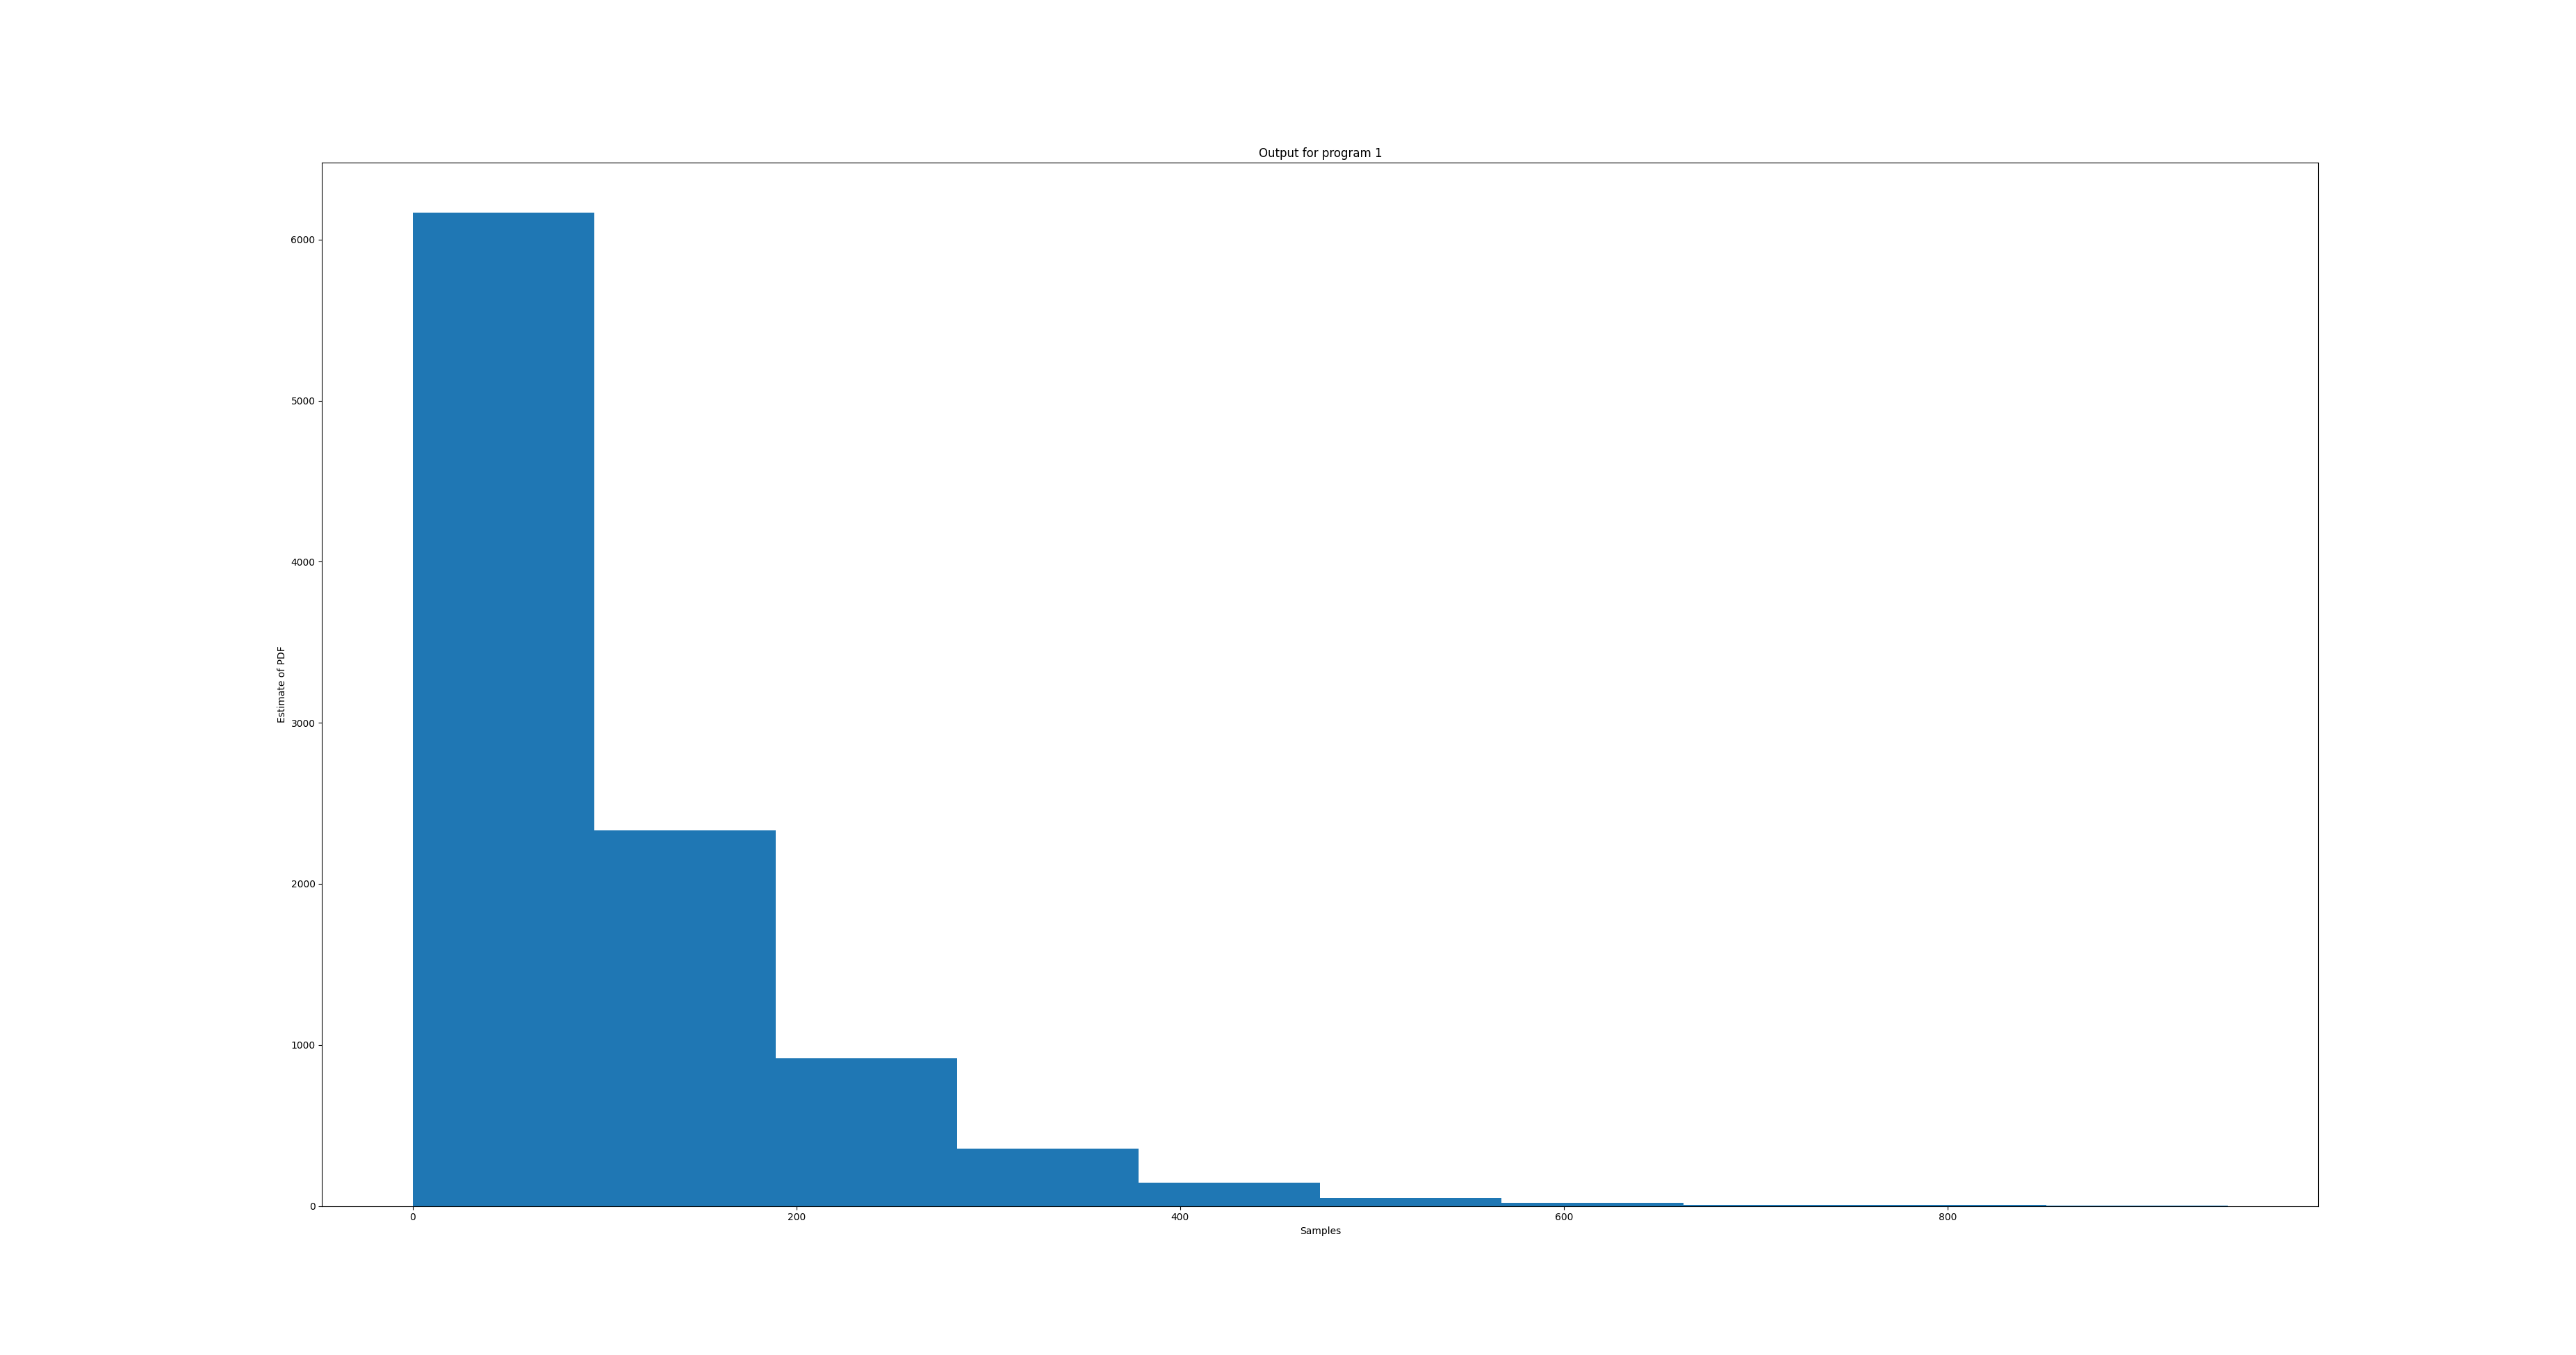
\includegraphics[width=\linewidth]{Figures/P1Hist.png}
	\captionof{figure}{Histogram for Program 1}
\end{center}

\subsection{Program 2}
Output from running program 2:
\begin{verbatim}
Sample of prior of program 2:
Elapsed time for program  2 .daphne is:  0:00:15.488580  seconds
Mean of samples:  tensor(0.9696)
Variance of samples:  tensor(5.0563)
\end{verbatim}
\begin{center}
	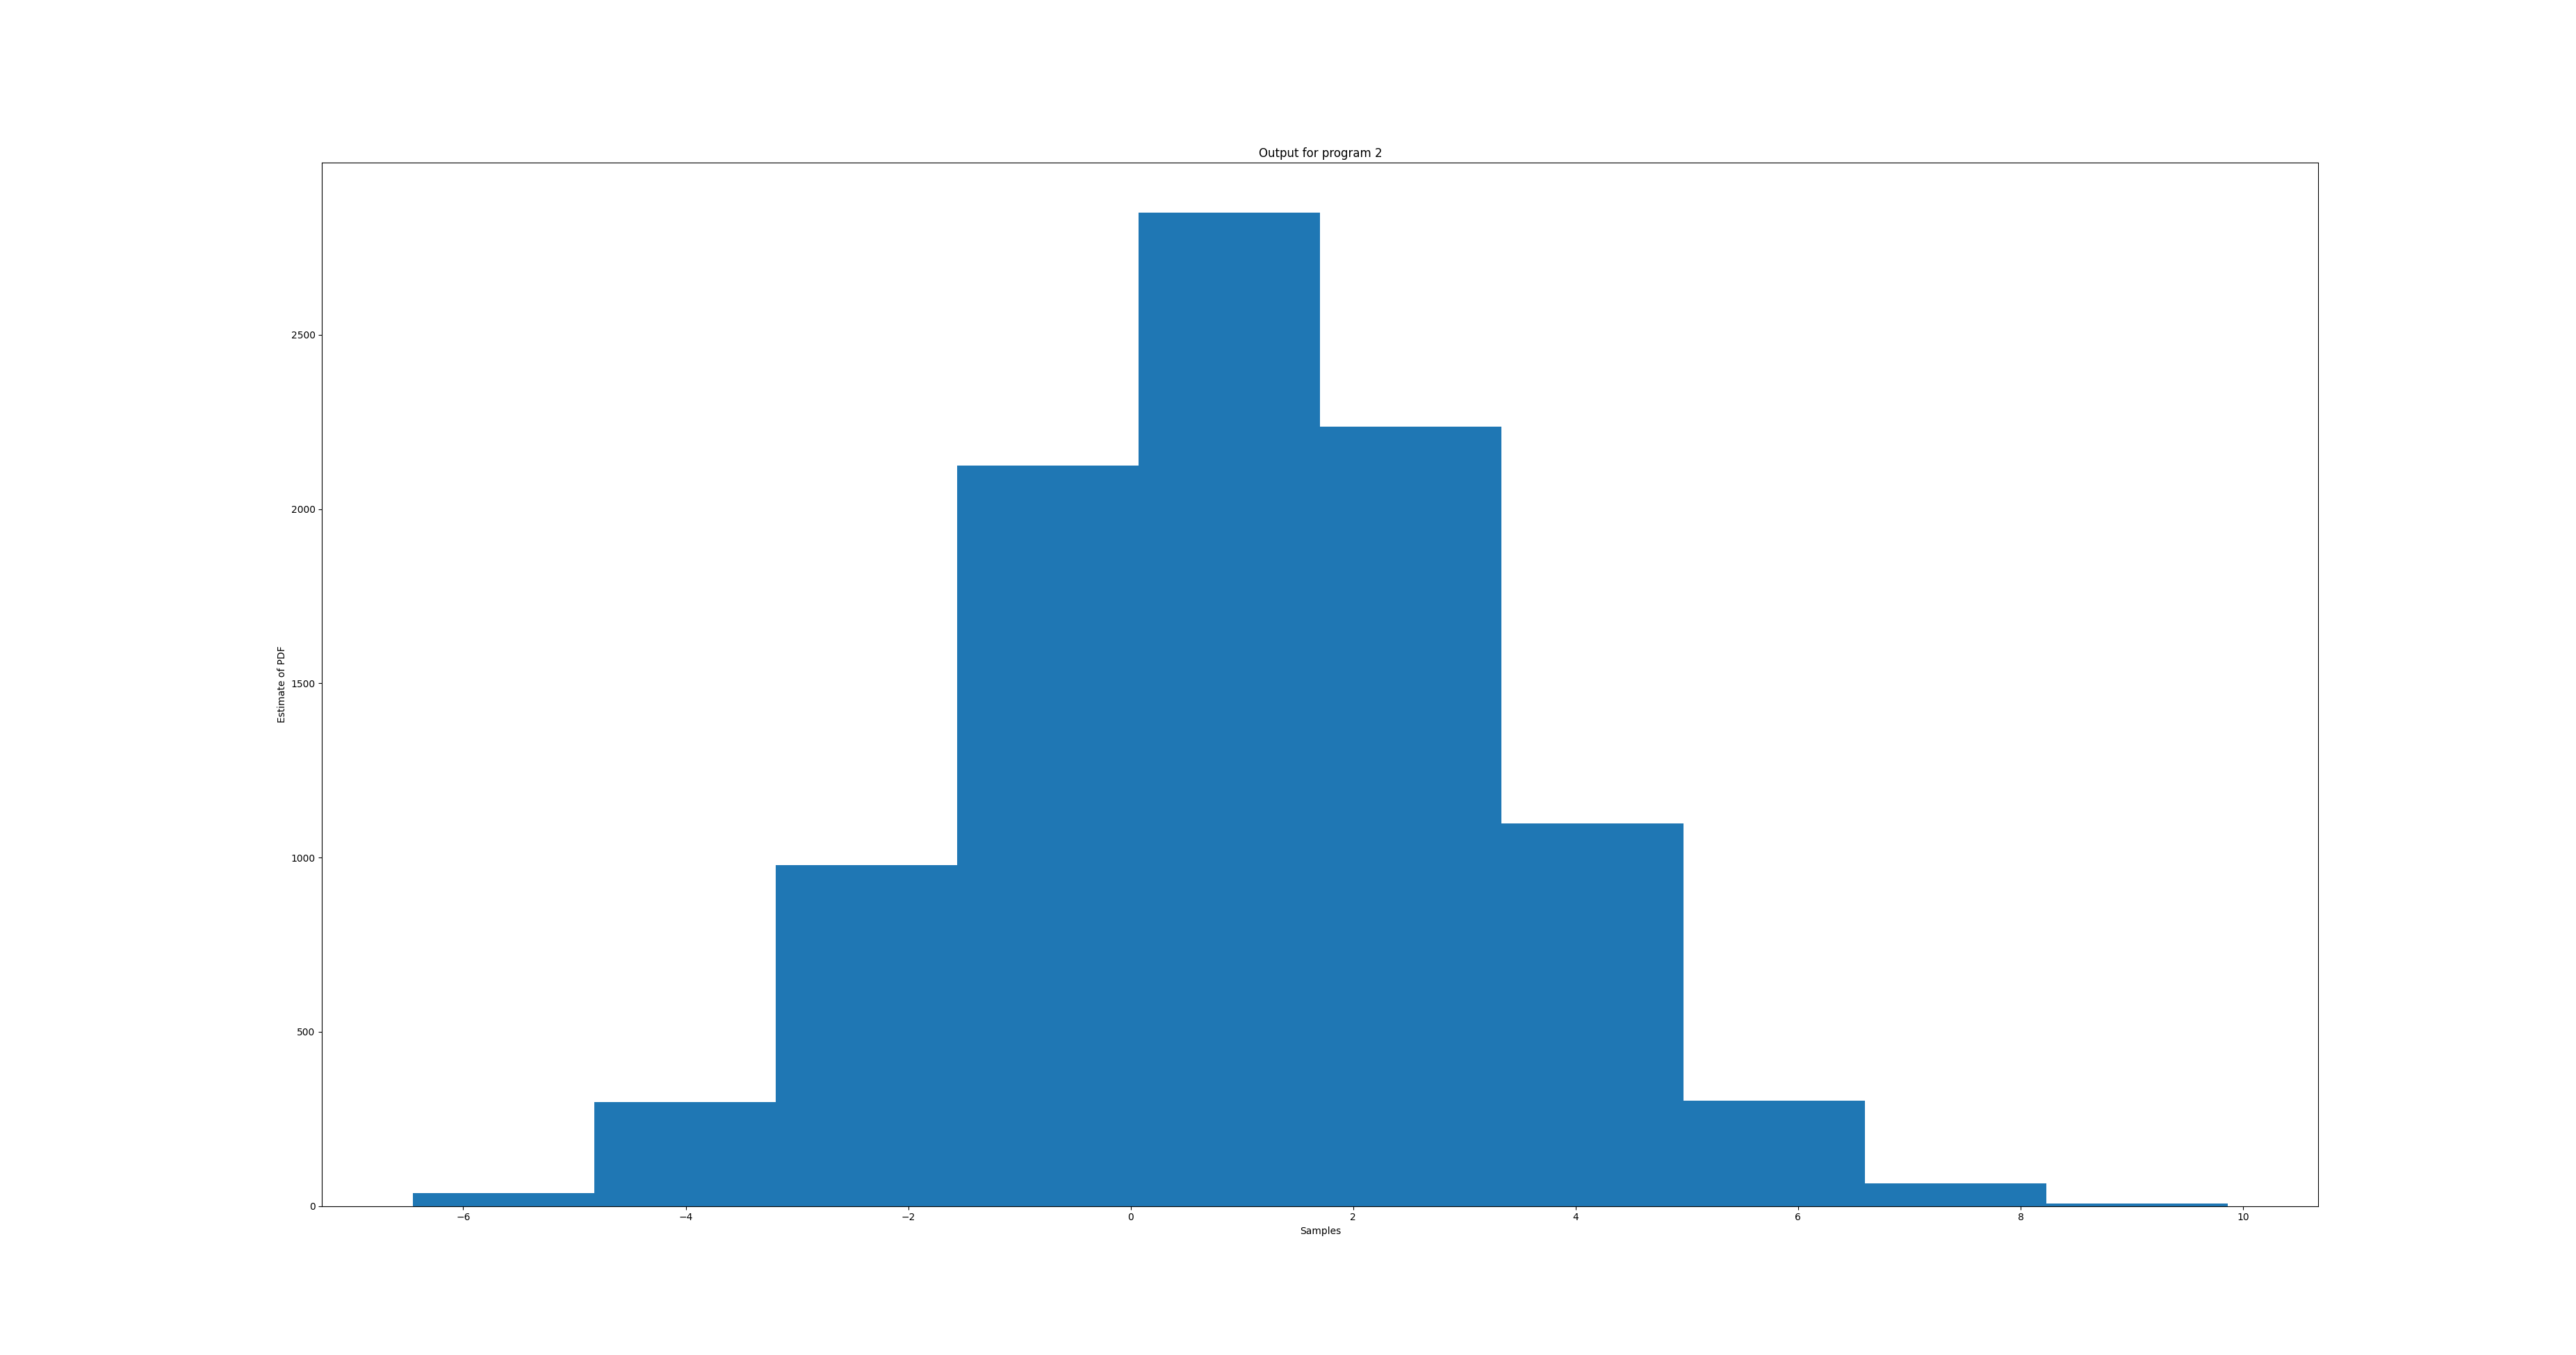
\includegraphics[width=\linewidth]{Figures/P2Hist.png}
	\captionof{figure}{Histogram for Program 2}
\end{center}

\subsection{Program 3}
Output from running program 3:
\begin{verbatim}
Sample of prior of program 3:
Elapsed time for program  3 .daphne is:  0:02:09.690632  seconds

\end{verbatim}
\begin{center}
	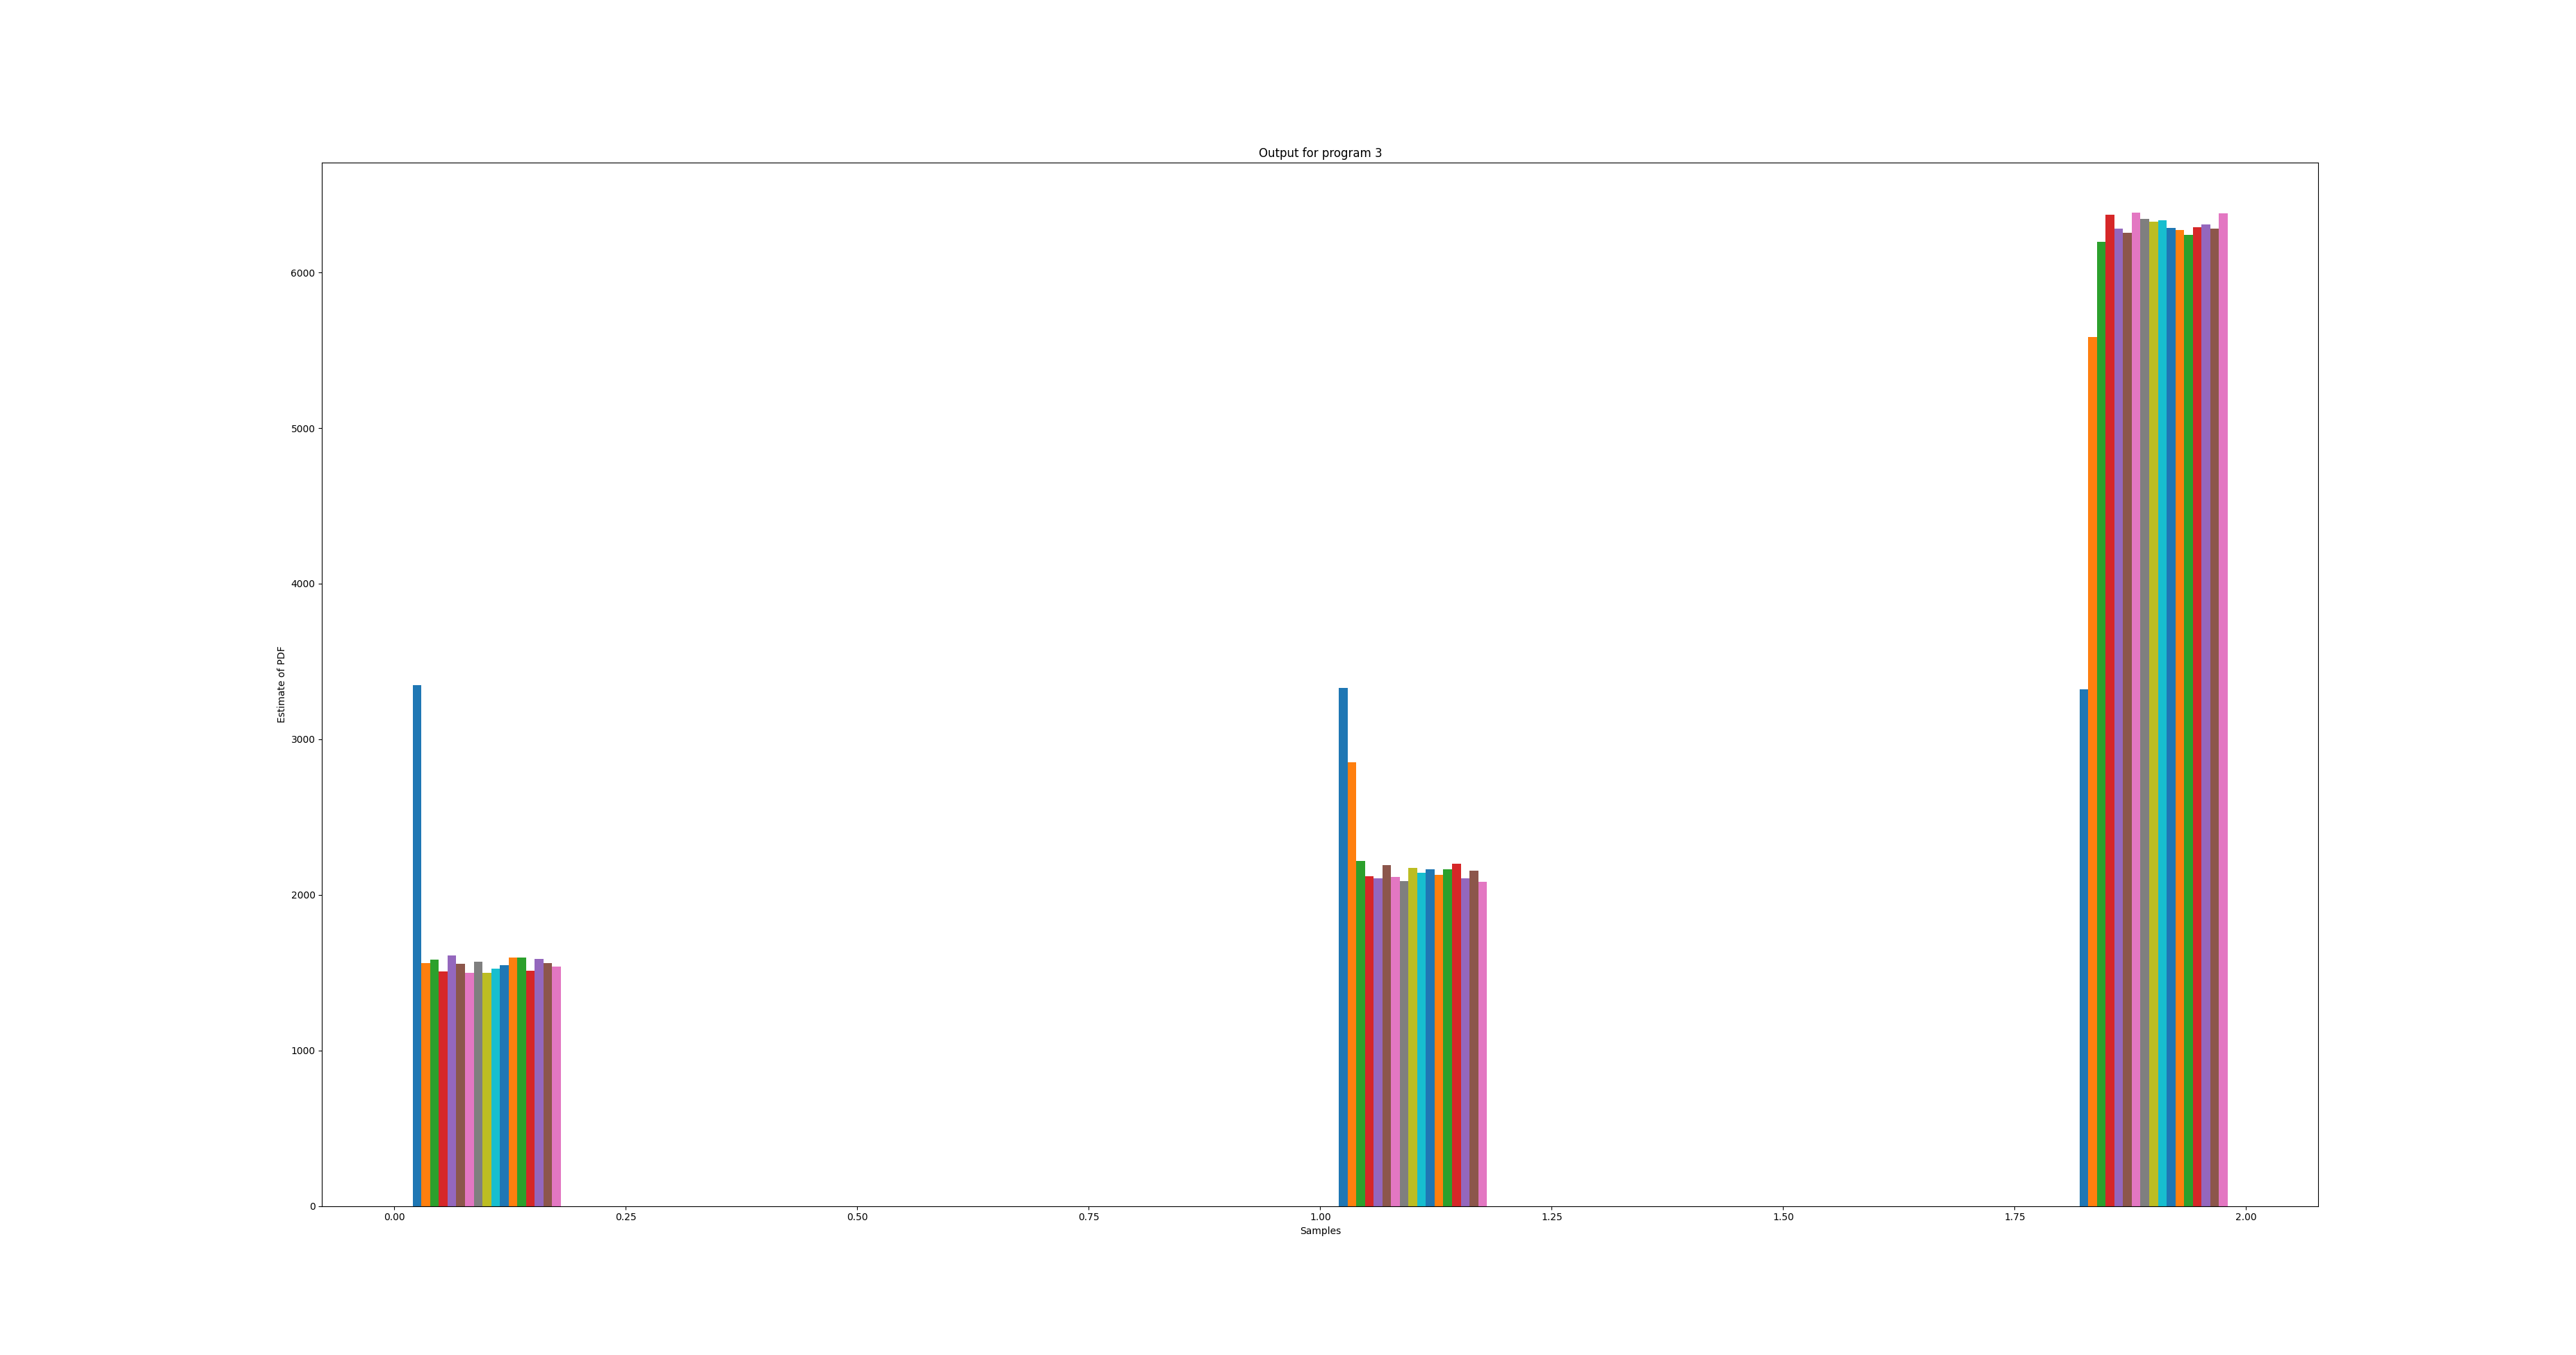
\includegraphics[width=\linewidth]{Figures/P3Hist.png}
	\captionof{figure}{Histogram for Program 3}
\end{center}
 
\end{document}
